\documentclass[a4paper,12pt,twocolumn]{article}
\usepackage[czech]{babel}
\usepackage[left=1.5cm,text={18cm, 25cm},top=2.5cm]{geometry}
\usepackage[IL2]{fontenc}
\usepackage[utf8]{inputenc}
\usepackage{svg, amsmath, amsthm, amssymb}

\begin{document}
\twocolumn[
	\begin{@twocolumnfalse}
		\begin{center}
			{\Large ISS Projekt 2018/19}\\
			\vspace*{5px}
			Matej Soroka $<$xsorok02$>$ \\
			\vspace*{10px}
		\end{center}
	\end{@twocolumnfalse}
]
\begin{enumerate}
\item
Vzorkovacia frekvencia signálu: 16000Hz\\
Dĺžka vo vzorkách: 32000\\
Dĺžka v sekundách: 2\\
Počet binárnych symbolov: 2000
\item
Signál preiterujem, s tým rozdielom že sa na začiatku posuniem o 8 vzoriek, a následne sa posuvám o 16 vzoriek po každej iterácii. V každej iterácii taktiež vyhodnocujem binárnu hodnotu podľa hodnoty signálu v danom bode a ukladám ju do poľa.
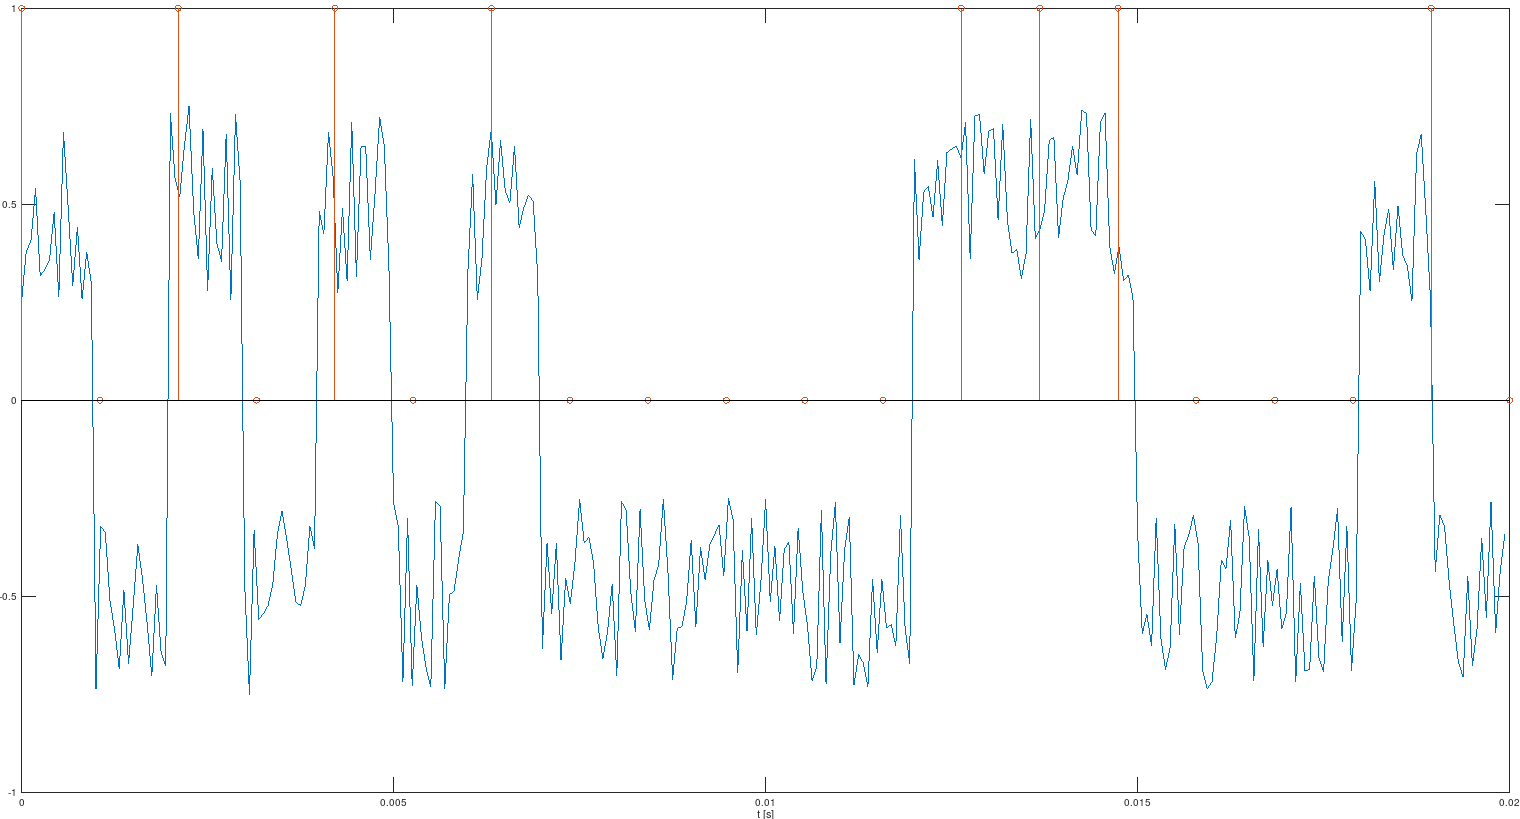
\includegraphics[width=\linewidth]{2}
\item
Filter je \textbf{stabilný}, všetky póly sú vo vnútri jednotkovej kružnice, graf som vytvoril pomocou funkcie \texttt{zplane}.
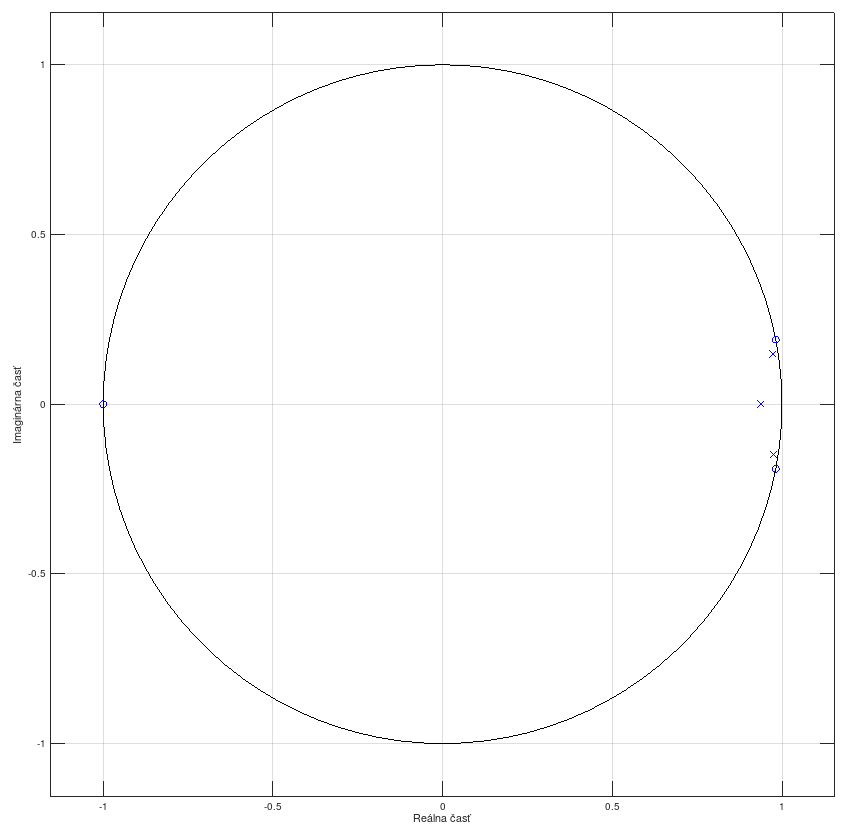
\includegraphics[width=\linewidth]{3}
\newpage
\item
Filter je typu \textbf{dolná priepusť}, ako vidíme v grafe. Medzná frekvencia je 487.25Hz.
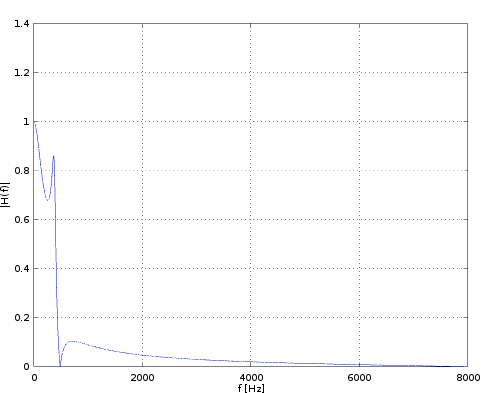
\includegraphics[width=\linewidth]{4}
\item
Využil som oneskorenie o 15 vzorkov. Snažil som sa o pretnutie osi x približne v čase 0.012s
\item
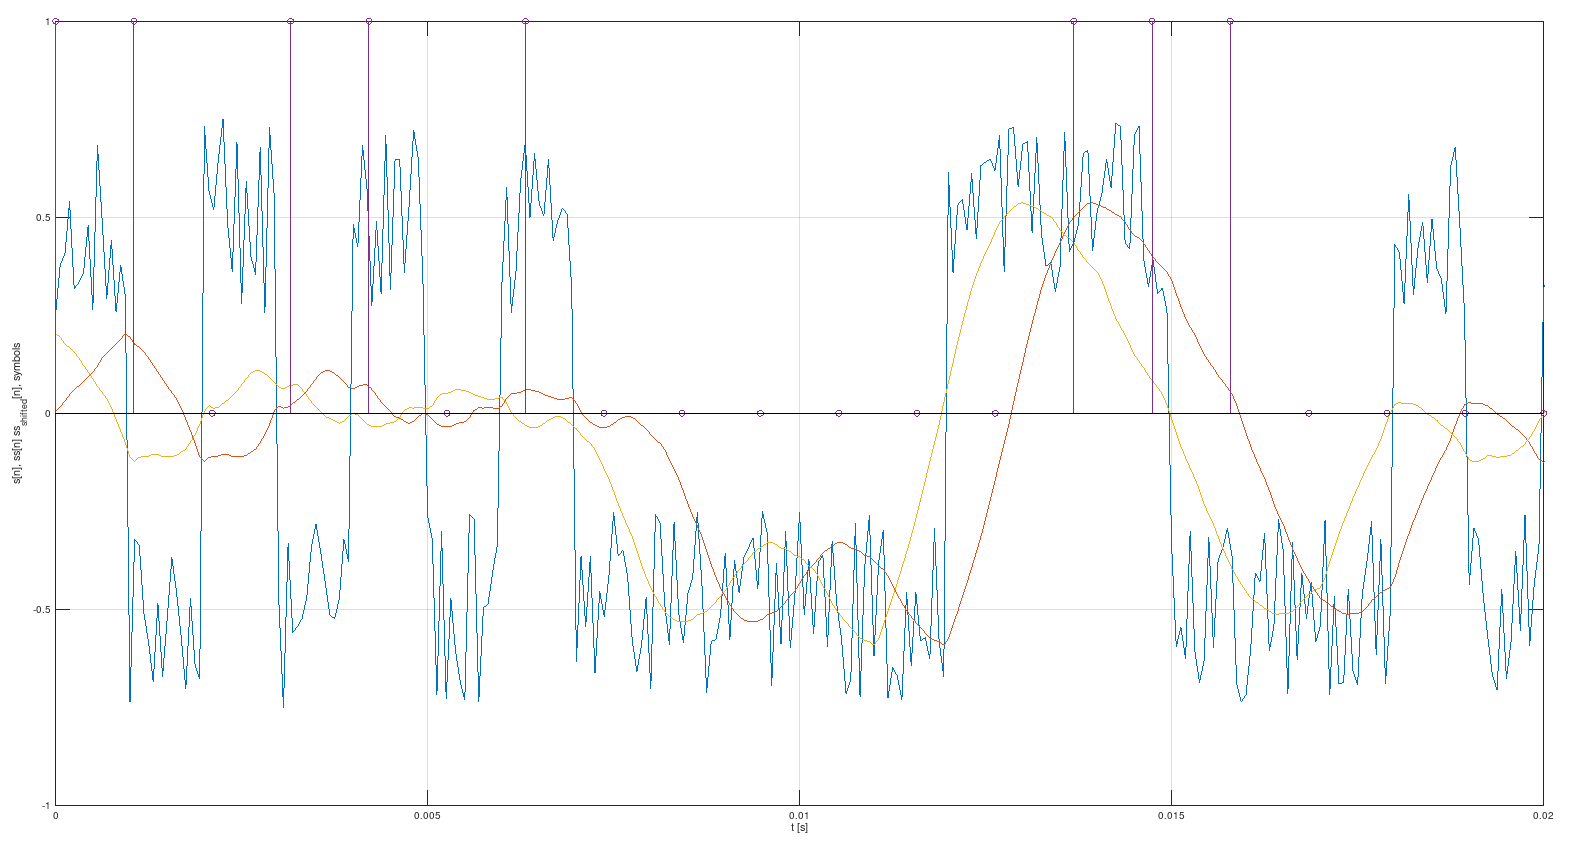
\includegraphics[width=\linewidth]{6}
\item
Kedže som signál posunul o viac ako 8 vzoriek, využil som o jednu vzorku menej.\\
Počet chýb: 1999\\
Celkový počet vzorkov: 83\\
Chybovosť: 4.1521
\newpage
\item
Filtrovaný signál sa približuje k nule omnoho rýchlejšie, takmer okamžite po medznej frekvecnii, po ktorej stagnuje.
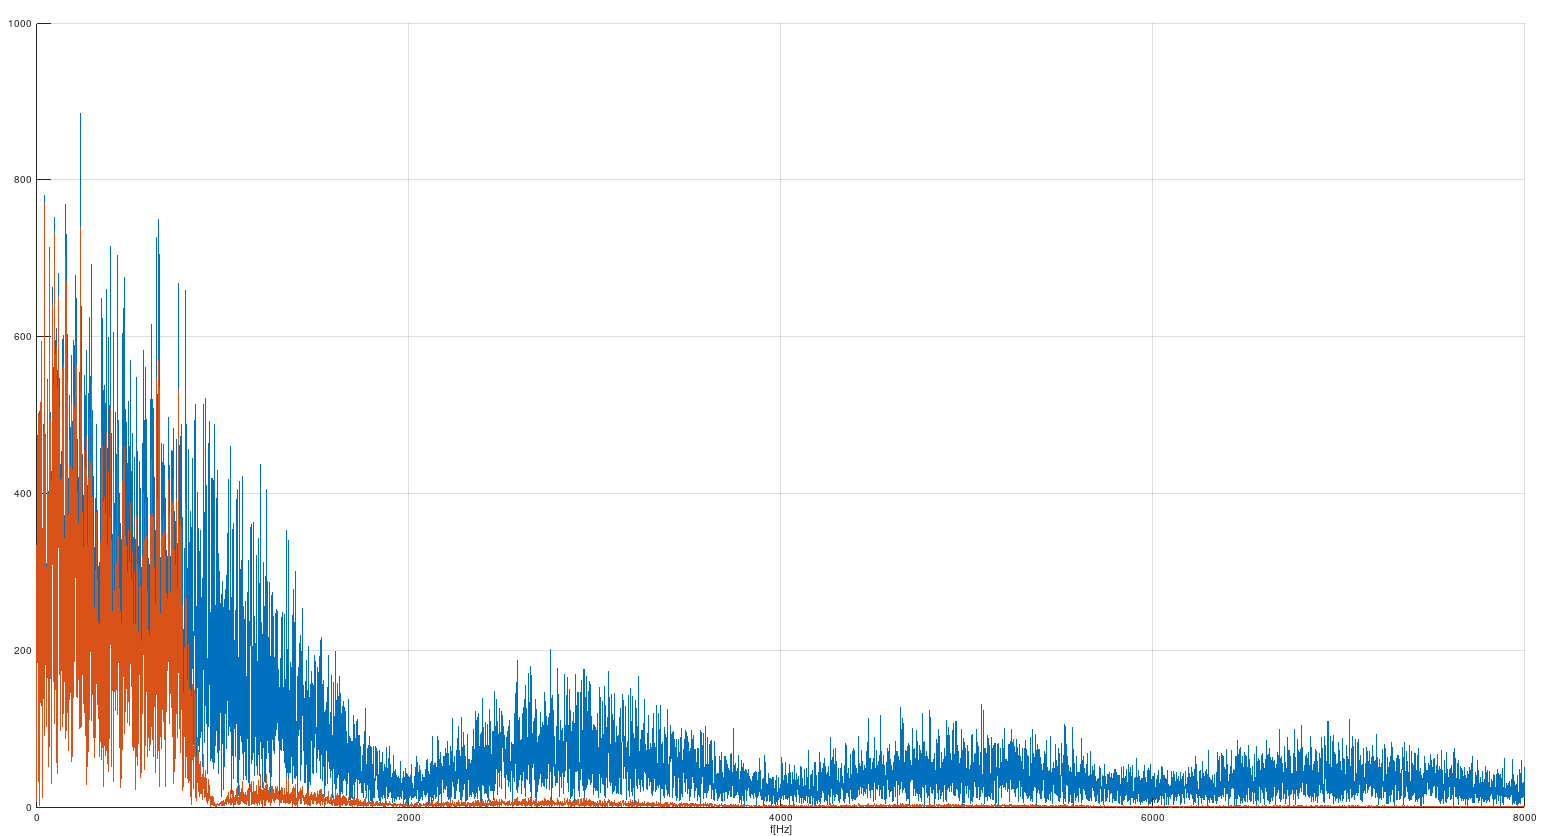
\includegraphics[width=\linewidth]{8}
\item
Použitá funkcia \texttt{hist} s načítaným signálom.
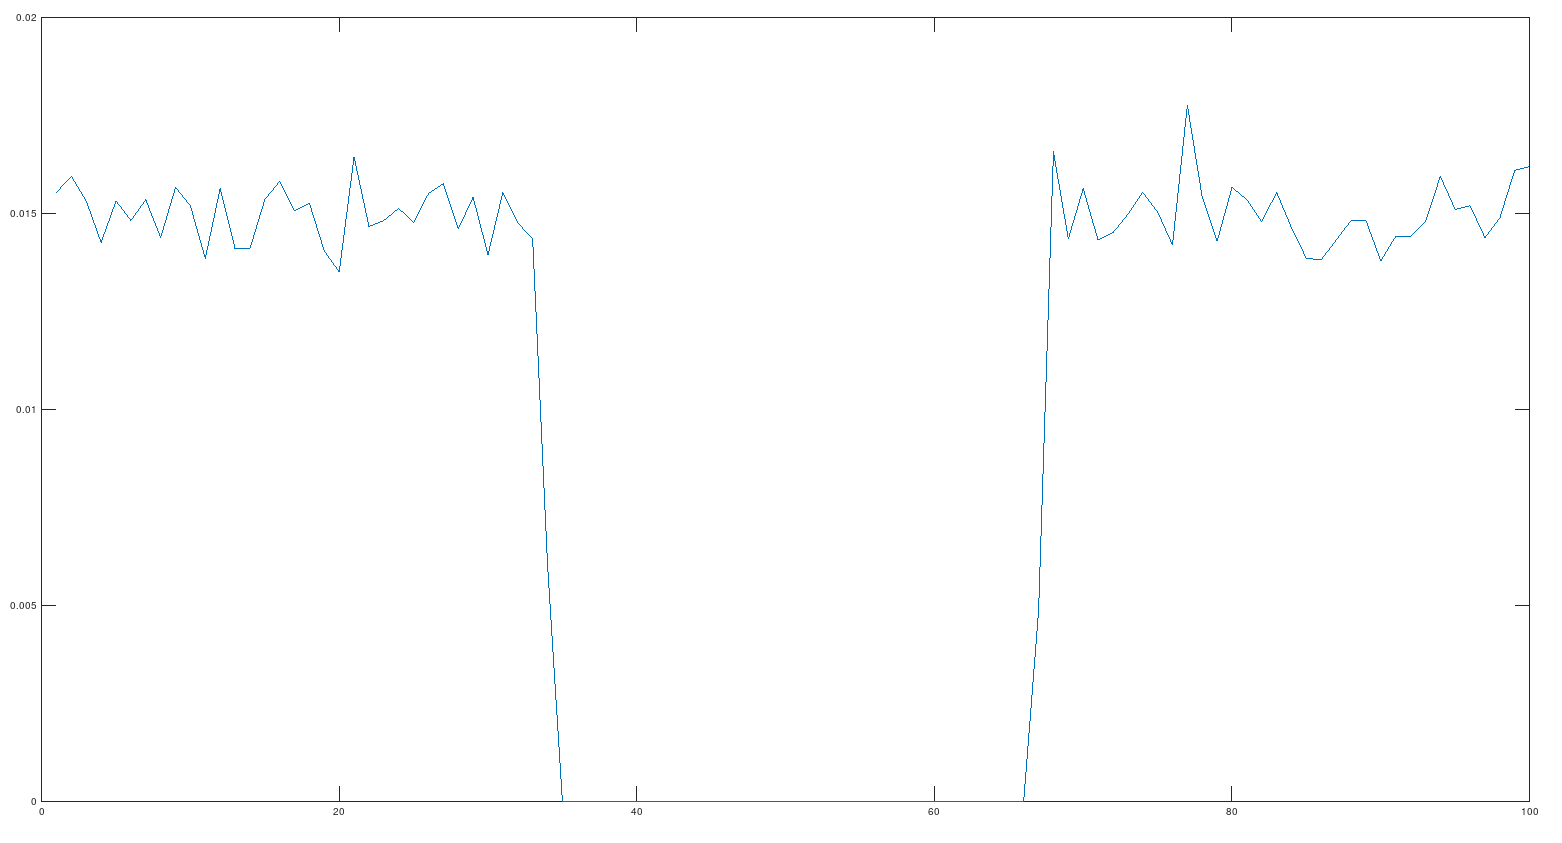
\includegraphics[width=\linewidth]{9}
\item
\texttt{[r, delay] = xcorr(s, 'biased');} Osa x limitovaná na $<$-50,50$>$
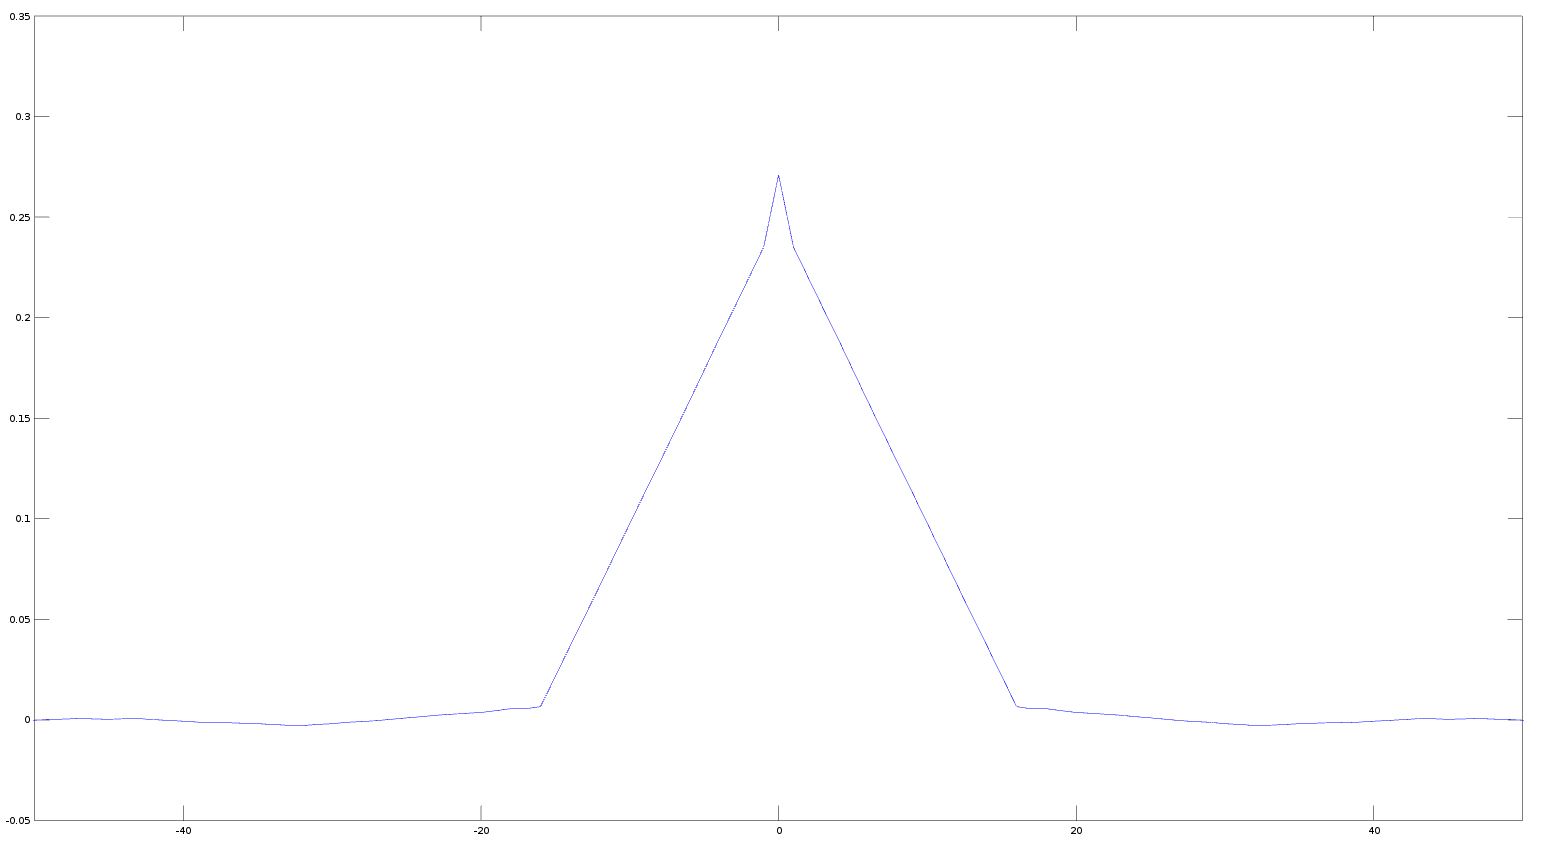
\includegraphics[width=\linewidth]{10}
\item
$R[0] = 0.27099 \\
R[1] = 0.097618 \\
R[16] = 0.0065915$
\item
Využil som funkciu hist2 a funkciu plot3.
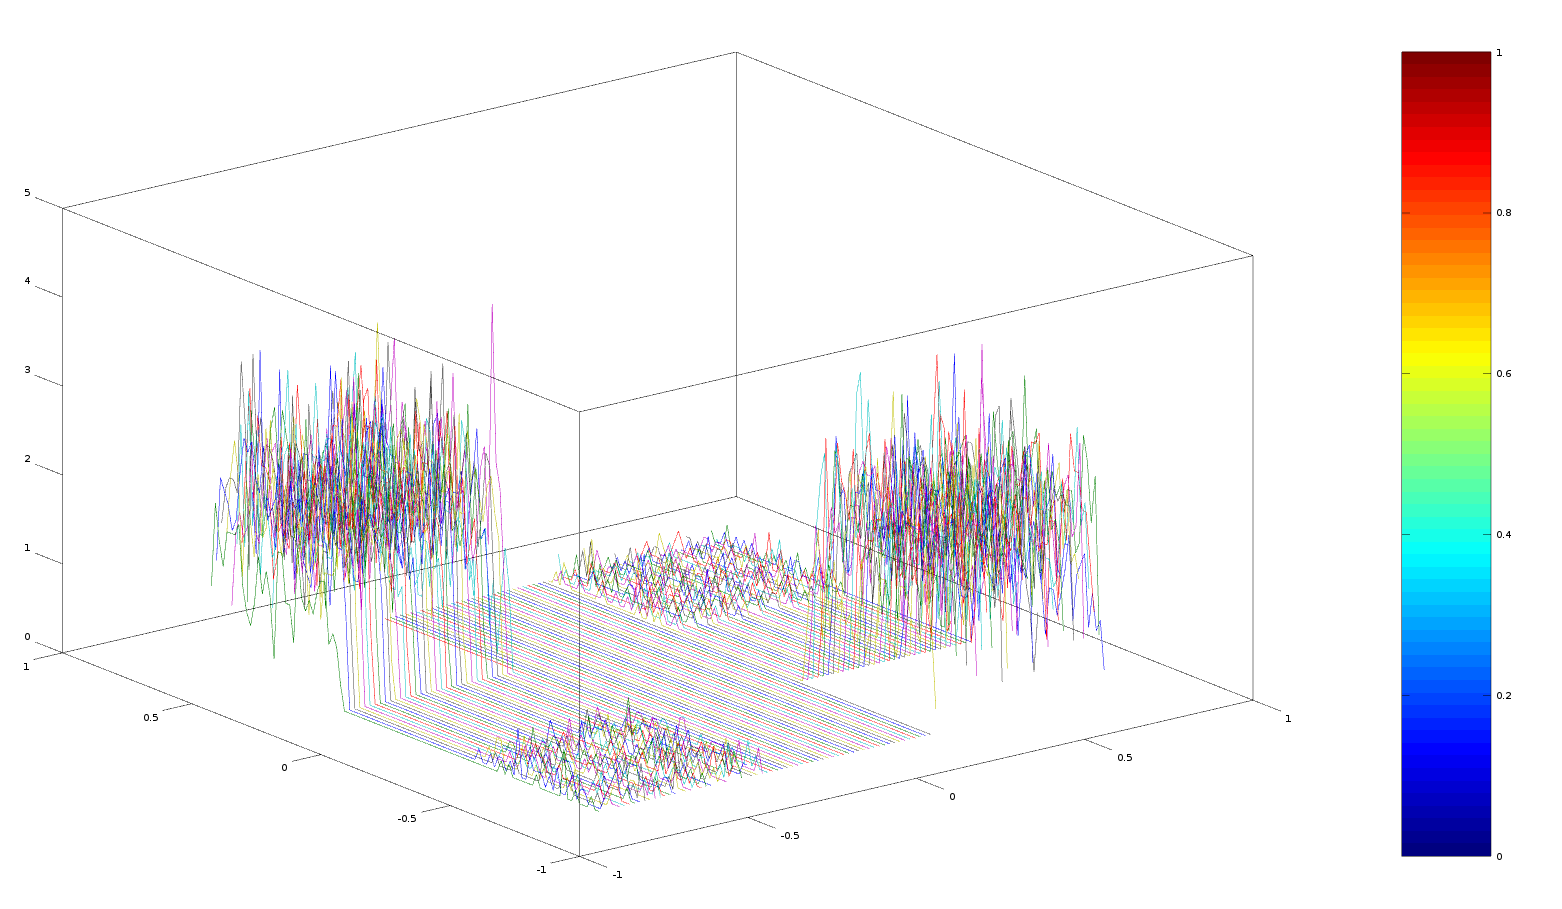
\includegraphics[width=\linewidth]{12}
\item
Overenie pomocou funkcie hist2 \\
\texttt{hist2: check -- 2d integral should be 1 and is 1}
\item
Výsledok funkcie hist2 je 0.235146 a R1 z úlohy 10. je 0.23513. S prijateľnou odchýlkou po zaokrúhlení sú tieto hodnoty rovnaké.
\end{enumerate}
\end{document}
